\documentclass[landscape,paperwidth=40in,paperheight=32in]{baposter}

\usepackage{graphicx}
\usepackage{enumitem}
\usepackage{url}
\usepackage{amssymb}
\usepackage[font=small,labelfont=bf]{caption}
\usepackage{multicol}

% This prevents a \section being created for the bibliography
\renewcommand{\section}[2]{}%

\newcommand{\BI}{\begin{itemize}[itemsep=.03in,parsep=0in,leftmargin=.2in]}
\newcommand{\EI}{\end{itemize}}

\newcommand{\BE}{\begin{enumerate}[itemsep=.03in,parsep=0in,leftmargin=.2in]}
\newcommand{\EE}{\end{enumerate}}

\definecolor{ycp}{RGB}{3,165,92}
\definecolor{gt}{RGB}{212,157,20}

\begin{document}

\begin{poster}{
  % key=value Options
  columns=4,
  colspacing=2em,
  headerheight=0.105\textheight,
  background=plain,
  bgColorOne=white,
  borderColor=black,
  headerColorOne=ycp,
  headershade=plain,
  headershape=roundedright,
  headerborder=closed,
  headerfont=\Large\bf,
  headerFontColor=white,
  textborder=roundedleft,
  boxshade=plain,
  boxColorOne=gt!25!white,
  linewidth=1pt
}{
  
\includegraphics[height=5em]{nsf1} \\
}{
  {\huge PhysiCloud: A Cloud-computing Platform for Cyber-physical Systems}
}{
  \vskip .05in
  {\large
 	Paul Glotfelter, Patrick J. Martin - York College of Pennsylvania \\
  \smallskip
  www.ycp.edu
  }
}{
  \includegraphics[height=5em]{hypower-logo-final}
}

%---------------------------------
% Project Goals
%---------------------------------  
  \headerbox{Project Goals}{name=goals,column=0,span=1}{
%  	\vskip .1in
	{\raggedright\normalsize
	\BI
		\item Develop light-weight cloud-computing platform 
		\item Eliminate networking complexities
		\item Allow student use (better point)
	\EI
	}
  }
  
%---------------------------------
% Personnel
%---------------------------------  
  \headerbox{Personnel}{name=personnel,column=0,span=1,below=goals}{
%  	\vskip .1in
	{\raggedright\normalsize
	A collaborative effort among faculty and students at York College of Pennsylvania: \\ \medskip
	{\bf Faculty} \\
	
	Patrick J. Martin - CPS cloud computing \\	
	\medskip	
	
	{\bf Undergraduate Students} \\
	
	Travis Eichelberger \\
	Paul Glotfelter \\ 
	Samuel Nelson

	}
  }

%---------------------------------
% Current Developments
%---------------------------------  

%\headerbox{Performance Regulation for Multi-Core Processors}{name=perfreg,column=1,span=3,row=0,below=poweraware-mob}{
\headerbox{Project Results}{name=proj-results,column=1,span=3,row=0, above=bottom, aligned=goals}{

{\bf\large Framework}
    
	\begin{minipage}[t]{0.80\linewidth}
	
		PhysiCloud is a cyber-physical, cloud-computing infrastructure. \\
		
		\begin{minipage}{0.5\linewidth}
    			\BI
				\item Enables cloud-computing on low-power, mobile systems.
				\item Facilitates simple access to cyber-physical resources.
				\item Provides resiliency to network and power failures.
			\EI	
		\end{minipage}		
		~~~~~~~~	~~~~~
		\begin{minipage}{0.66\linewidth}
			    	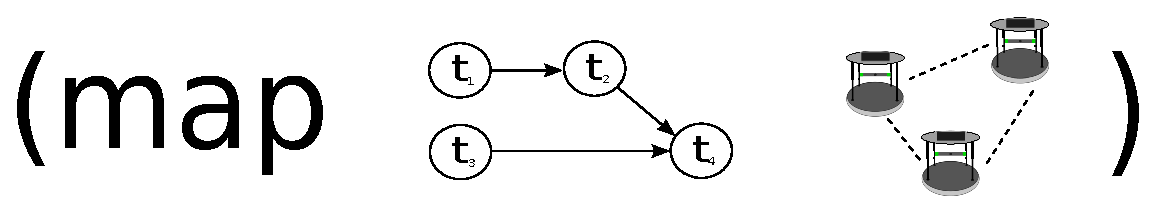
\includegraphics[width=\linewidth]{project-objective}
   	 	\end{minipage}	
    \end{minipage}
    
%    \begin{minipage}[t]{0.80\linewidth}
%    		\begin{minipage}{0.55\linewidth}
%    			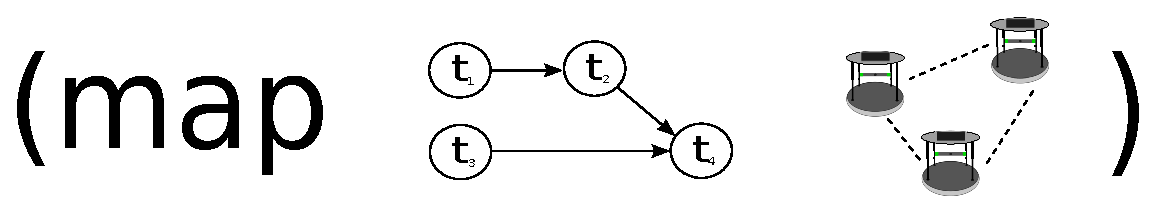
\includegraphics[width=\linewidth]{project-objective}
%   	 	\end{minipage}	  
%    \end{minipage}
    	
\vspace{1.5em}

{\bf\large Tasks}

	\smallskip

  	\begin{minipage}[t]{0.80\linewidth}
	
		To facilitate the programming of an application, PhysiCloud provides a task and channel interface based on Communicating Sequential Processes (CSP).
		
		\smallskip
		
		\begin{minipage}{0.5\linewidth}
    			\BI
				\item Clarifies data-flow of application
				\item Allows distribution of tasks
				\item Most control applications can be easily modelled by CSP
			\EI	
		\end{minipage}		
		\begin{minipage}{0.7\linewidth}
			    	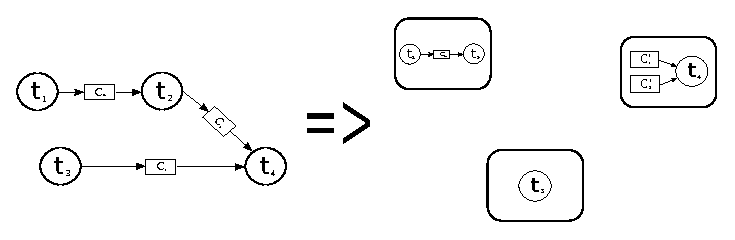
\includegraphics[width=\linewidth]{physicloud-tasks}
   	 	\end{minipage}	
    \end{minipage}
	
\vspace{1em}

{\bf\large Network Topology Construction}

	\smallskip

  	\begin{minipage}[t]{0.80\linewidth}
	
		PhysiCloud constructs a network topology such that all dependencies are satisfied.  This result is achieved by a two-phase process.
		
		\smallskip
		
		\begin{minipage}{0.5\linewidth}
    			\BI
				\item Clarifies data-flow of application
				\item Allows distribution of tasks
				\item Most control applications can be easily modelled by CSP
			\EI	
		\end{minipage}		
		~~~~~~
		\begin{minipage}{0.35\linewidth}
			    	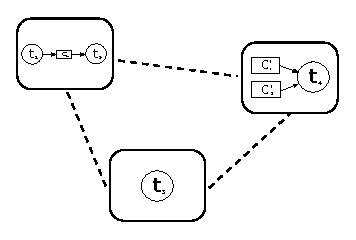
\includegraphics[width=\linewidth]{physicloud-udp}
   	 	\end{minipage}	
    \end{minipage}

	\bigskip

  	\begin{minipage}[t]{0.80\linewidth}
	
		The Monitor establishes TCP connections to each of the units and routes data appropriately.
		
		\bigskip
		
		\begin{minipage}{0.5\linewidth}
    			\BI
				\item Enables 
				\item Allows distribution of tasks
				\item Most control applications can be easily modelled by CSP
			\EI	
		\end{minipage}		
		~~~~~~
		\begin{minipage}{0.50\linewidth}
			    	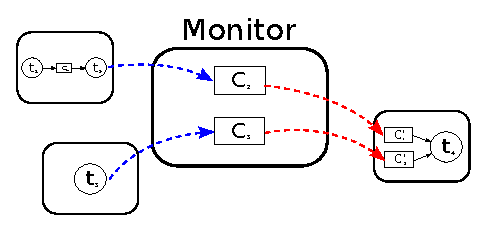
\includegraphics[width=\linewidth]{physicloud-monitor}
   	 	\end{minipage}	
    \end{minipage}
	
\vspace{1em}

}


%---------------------------------
% Contact
%---------------------------------

  \headerbox{Contact Information}{name=contacts,column=0,below=personnel}{
%    \vskip .1in
    {\raggedright\normalsize
%	{\bf Web:} hypower.gatech.edu \\
%    \smallskip
	{\bf Email:} \\
%    \BI
		pjmartin@ycp.edu \\
		pglotfel@ycp.edu
%    \EI
	}
  }

%---------------------------------
% Remaining work
%---------------------------------
  \headerbox{Future Work}{name=remaining,below=personnel,column=0,span=1}{
%    \vskip .1in
    {\raggedright\normalsize
    \BI
    		\item Hybrid centralized/decentralized optimization, coordination, and control design using the PhysiCloud architecture
		\item Development of GUI
		\item Cross-platform/language operability
    \EI
    }
  }

%---------------------------------
% Acknowledgements
%---------------------------------

  \headerbox{Acknowledgements}{name=acks,column=0,below=remaining}{
%    \vskip .1in
    {\raggedright\normalsize
    This work is funded by the following NSF Grants:
    \BI
    	\item CNS-1239221
		\item CNS-1239225
    \EI}
  }


\end{poster}

\end{document}
